%%%%%%%%%%%%%%%%%%%%%%%%%%%%%%%%%%%%%%%%%
% Programming/Coding Assignment
% LaTeX Template
%
% This template has been downloaded from:
% http://www.latextemplates.com
%
% Original author:
% Ted Pavlic (http://www.tedpavlic.com)
%
% Note:
% The \lipsum[#] commands throughout this template generate dummy text
% to fill the template out. These commands should all be removed when 
% writing assignment content.
%
% This template uses a Perl script as an example snippet of code, most other
% languages are also usable. Configure them in the "CODE INCLUSION 
% CONFIGURATION" section.
%
%%%%%%%%%%%%%%%%%%%%%%%%%%%%%%%%%%%%%%%%%

%----------------------------------------------------------------------------------------
%	PACKAGES AND OTHER DOCUMENT CONFIGURATIONS
%----------------------------------------------------------------------------------------

\documentclass{article}

\usepackage{fancyhdr} % Required for custom headers
\usepackage{lastpage} % Required to determine the last page for the footer
\usepackage{extramarks} % Required for headers and footers
\usepackage[usenames,dvipsnames]{color} % Required for custom colors
\usepackage{graphicx} % Required to insert images
\usepackage{listings} % Required for insertion of code
\usepackage{courier} % Required for the courier font
\usepackage{lipsum} % Used for inserting dummy 'Lorem ipsum' text into the template
\usepackage{epstopdf} % Convert Matlab figures to pdf
\usepackage{amsmath}
\usepackage{esint}
\usepackage{cancel}
\usepackage{amssymb}

% Margins
\topmargin=-0.45in
\evensidemargin=0in
\oddsidemargin=0in
\textwidth=6.5in
\textheight=9.0in
\headsep=0.25in

\linespread{1.1} % Line spacing

% Set up the header and footer
\pagestyle{fancy}
\lhead{\hmwkAuthorName} % Top left header
\chead{\hmwkClass\ (\hmwkClassInstructor): \hmwkTitle} % Top center head
\rhead{\firstxmark} % Top right header
\lfoot{\lastxmark} % Bottom left footer
\cfoot{} % Bottom center footer
\rfoot{Page\ \thepage\ of\ \protect\pageref{LastPage}} % Bottom right footer
\renewcommand\headrulewidth{0.4pt} % Size of the header rule
\renewcommand\footrulewidth{0.4pt} % Size of the footer rule

\setlength\parindent{0pt} % Removes all indentation from paragraphs

%----------------------------------------------------------------------------------------
%	CODE INCLUSION CONFIGURATION
%----------------------------------------------------------------------------------------

\definecolor{MyDarkGreen}{rgb}{0.0,0.4,0.0} % This is the color used for comments
\lstloadlanguages{Python} % Load Python syntax for listings, for a list of other languages supported see: ftp://ftp.tex.ac.uk/tex-archive/macros/latex/contrib/listings/listings.pdf
\lstset{language=Python, % Use Python
        frame=single, % Single frame around code
        basicstyle=\small\ttfamily, % Use small true type font
        keywordstyle=[1]\color{Blue}\bf, % Matlab functions bold and blue
        keywordstyle=[2]\color{Purple}, % Matlab function arguments purple
        keywordstyle=[3]\color{Blue}\underbar, % Custom functions underlined and blue
        identifierstyle=, % Nothing special about identifiers                                         
        commentstyle=\usefont{T1}{pcr}{m}{sl}\color{MyDarkGreen}\small, % Comments small dark green courier font
        stringstyle=\color{Purple}, % Strings are purple
        showstringspaces=false, % Don't put marks in string spaces
        tabsize=5, % 5 spaces per tab
        %
        % Put standard Python functions not included in the default language here
        morekeywords={rand,logrnd,var,mode,skewness,kurtosis},
        %
        % Put function parameters here
        morekeywords=[2]{on, off, interp},
        %
        % Put user defined functions here
        morekeywords=[3]{test},
       	%
        morecomment=[l][\color{Blue}]{...}, % Line continuation (...) like blue comment
        numbers=left, % Line numbers on left
        firstnumber=1, % Line numbers start with line 1
        numberstyle=\tiny\color{Blue}, % Line numbers are blue and small
        stepnumber=5 % Line numbers go in steps of 5
}

% Creates a new command to include a script, the first parameter is the filename of the script (without .m), the second parameter is the caption
\newcommand{\script}[5]{
\begin{itemize}
\item[]\lstinputlisting[caption=#2,label=#1,firstline=#3,lastline=#4,firstnumber=#5]{#1.py}
\end{itemize}
}

%----------------------------------------------------------------------------------------
%	DOCUMENT STRUCTURE COMMANDS
%	Skip this unless you know what you're doing
%----------------------------------------------------------------------------------------

% Header and footer for when a page split occurs within a problem environment
\newcommand{\enterProblemHeader}[1]{
\nobreak\extramarks{#1}{#1 continued on next page\ldots}\nobreak
\nobreak\extramarks{#1 (continued)}{#1 continued on next page\ldots}\nobreak
}

% Header and footer for when a page split occurs between problem environments (seems to be where listing the previous problem between problems is occurring)
\newcommand{\exitProblemHeader}[1]{
\nobreak\extramarks{#1 (continued)}{#1 continued on next page\ldots}\nobreak
\stepcounter{homeworkProblemCounter} % Increase counter for number of problems
\nobreak\extramarks{#1}{}\nobreak
}

\setcounter{secnumdepth}{0} % Removes default section numbers
\newcounter{homeworkProblemCounter} % Creates a counter to keep track of the number of problems
\addtocounter{homeworkProblemCounter}{1}

\newcommand{\homeworkProblemName}{}
\newenvironment{homeworkProblem}[1][Problem \arabic{homeworkProblemCounter}]{ % Makes a new environment called homeworkProblem which takes 1 argument (custom name) but the default is "Problem #"
%\stepcounter{homeworkProblemCounter} % Increase counter for number of problems
\renewcommand{\homeworkProblemName}{#1} % Assign \homeworkProblemName the name of the problem
\section{\homeworkProblemName} % Make a section in the document with the custom problem count
\enterProblemHeader{\homeworkProblemName} % Header and footer within the environment
}{
\exitProblemHeader{\homeworkProblemName} % Header and footer after the environment
}

\newcommand{\problemAnswer}[1]{ % Defines the problem answer command with the content as the only argument
\noindent\framebox[\columnwidth][c]{\begin{minipage}{0.98\columnwidth}#1\end{minipage}} % Makes the box around the problem answer and puts the content inside
}

\newcommand{\homeworkSectionName}{}
\newenvironment{homeworkSection}[1]{ % New environment for sections within homework problems, takes 1 argument - the name of the section
\renewcommand{\homeworkSectionName}{#1} % Assign \homeworkSectionName to the name of the section from the environment argument
\subsection{\homeworkSectionName} % Make a subsection with the custom name of the subsection
\enterProblemHeader{\homeworkProblemName\ [\homeworkSectionName]} % Header and footer within the environment
}{
\enterProblemHeader{\homeworkProblemName} % Header and footer after the environment
}

%----------------------------------------------------------------------------------------
%	NAME AND CLASS SECTION
%----------------------------------------------------------------------------------------

\newcommand{\hmwkTitle}{Homework\ \#5} % Assignment title
\newcommand{\hmwkDueDate}{Thursday,\ December\ 3,\ 2015} % Due date
\newcommand{\hmwkClass}{NUEN\ 629} % Course/class
\newcommand{\hmwkClassInstructor}{Ryan G. McClarren} % Teacher/lecturer
\newcommand{\hmwkAuthorName}{James B. Tompkins} % Your name

%----------------------------------------------------------------------------------------
%	TITLE PAGE
%----------------------------------------------------------------------------------------

\title{
\vspace{2in}
\textmd{\textbf{\hmwkClass:\ \hmwkTitle}}\\
\normalsize\vspace{0.1in}\small{\hmwkDueDate}\\
\vspace{0.1in}\large{\textit{\hmwkClassInstructor}}
\vspace{3in}
}

\author{\textbf{\hmwkAuthorName}}
\date{} % Insert date here if you want it to appear below your name

%----------------------------------------------------------------------------------------

\begin{document}

\maketitle

\clearpage
%----------------------------------------------------------------------------------------
%	PROBLEM 1
%----------------------------------------------------------------------------------------

% To have just one problem per page, simply put a \clearpage after each problem

\begin{homeworkProblem}

The requested activation and decay chains may be found in Cadwallader and Longhurst's 
1999 report (Cadwallader, L. \& Longhurst, G. (1999). FLiBe Use in Fusion Reactors: An Initial 
Safety Assessment. \textit{Idaho National Engineering and Environmental Laboratory.}).  The 
depletion calculations performed in subsequent problems primarily involves these activation and 
decay chains, but additional chains are considered for the listed products as well.

\begin{figure}[h!]
	\centering
		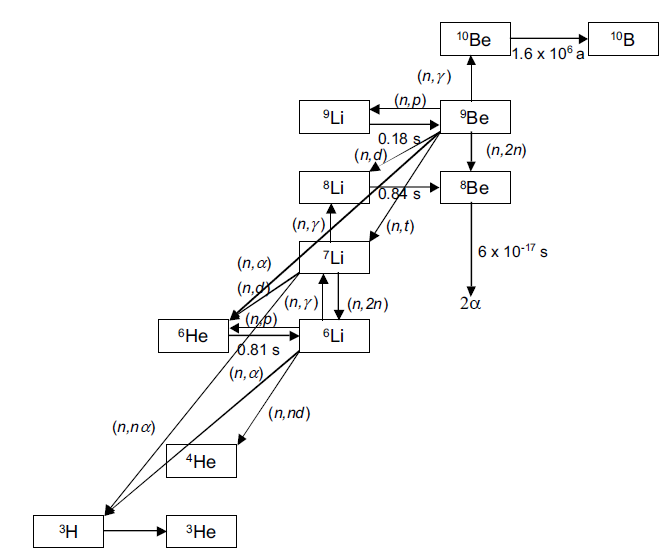
\includegraphics[width=.95\textwidth]{figures/1_1.png}
	\caption{Lithium and beryllium activation and decay chain (Cadwallader \& Longhurst)}
\end{figure}

\begin{figure}[h!]
	\centering
		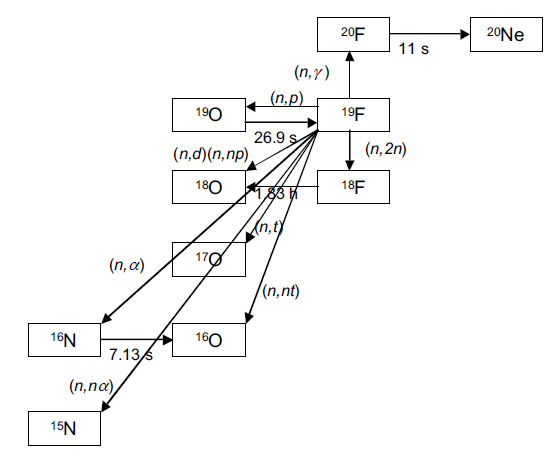
\includegraphics[width=.95\textwidth]{figures/1_2.png}
	\caption{Fluorine activation and decay chain (Cadwallader \& Longhurst)}
\end{figure}





\clearpage

\end{homeworkProblem}

%----------------------------------------------------------------------------------------
%	PROBLEM 2
%----------------------------------------------------------------------------------------

% To have just one problem per page, simply put a \clearpage after each problem

\begin{homeworkProblem}

We are asked to solve the given depletion problem by calculating the concentration of tritium
present in the FLiBe blanket around a fusion reactor after a two year irradation period.  First,
the cross sections and half lives of the nuclides involved in the decay chains are found using
OECD's Janis software, then creating an activation and decay matrix to use in finding the solution
to this problem.  The following listing details the backward Euler solution method.

\script{../hw5}{Backward Euler Solution Method}{304}{321}{304}

The calculated tritium concentration in the FLiBe blanket after two years of irradiation 
is 4.291837 x 10$^5$ kg tritium per kg FLiBe original material.  Thirty-three isotopes
were tracked in this simulation, and results over time for the fourteen nuclides with 
largest concentration at the end of the irradation cycle are given in Figures 3 and 4.

\clearpage

\begin{figure}[h!]
	\centering
		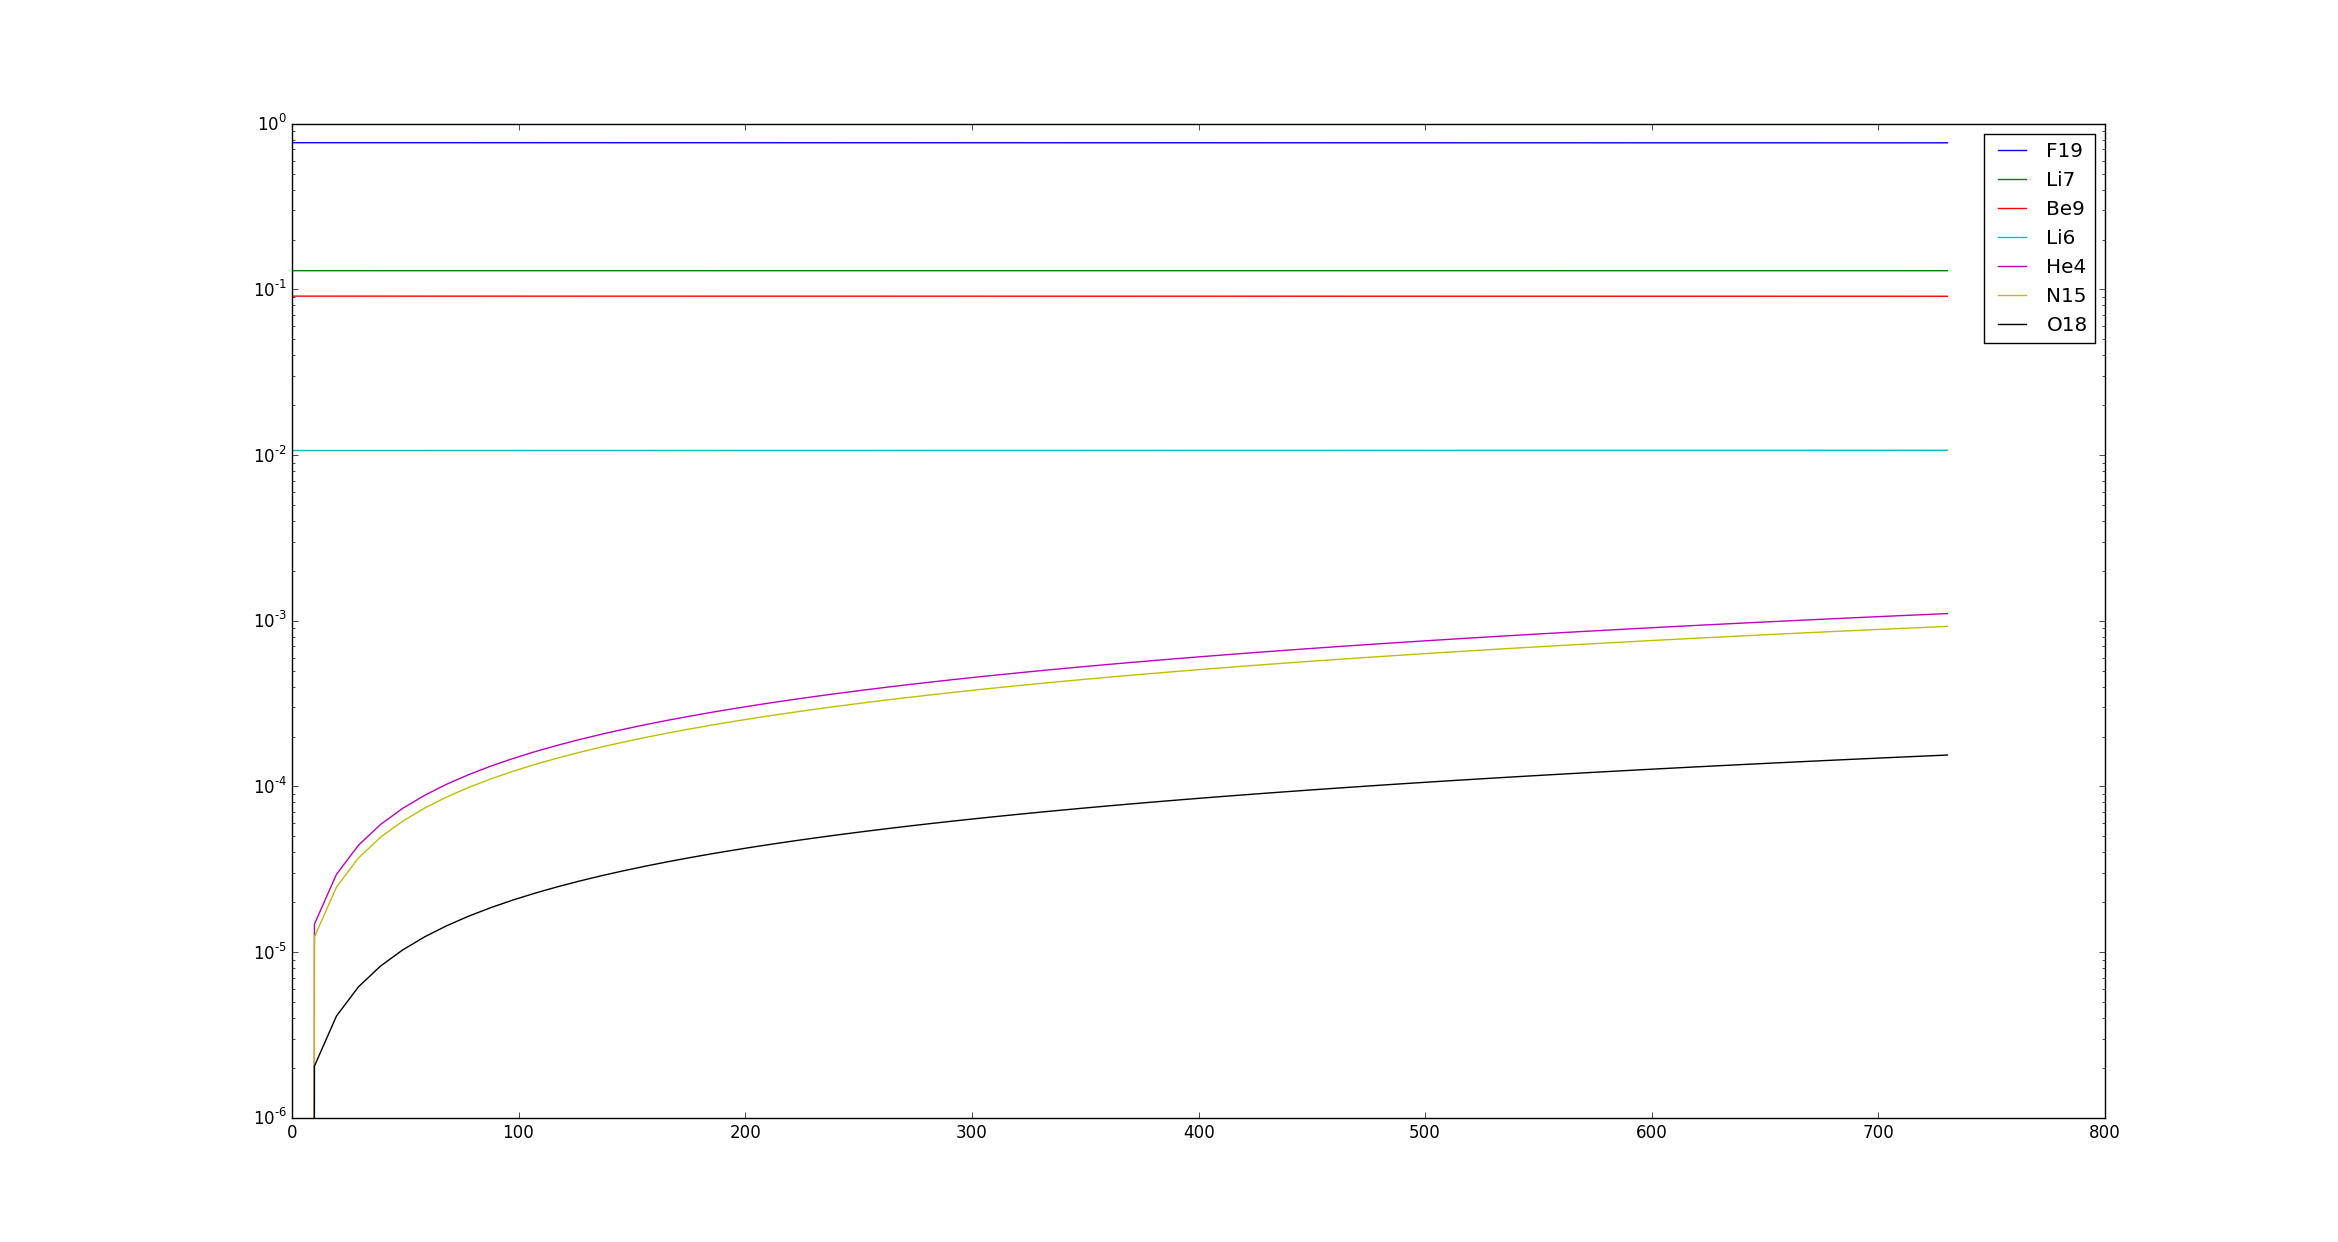
\includegraphics[width=.95\textwidth]{figures/2_1.png}
	\caption{Nuclides with largest concentration after the two year irradiation period from backward Euler method.}
\end{figure}

\begin{figure}[h!]
	\centering
		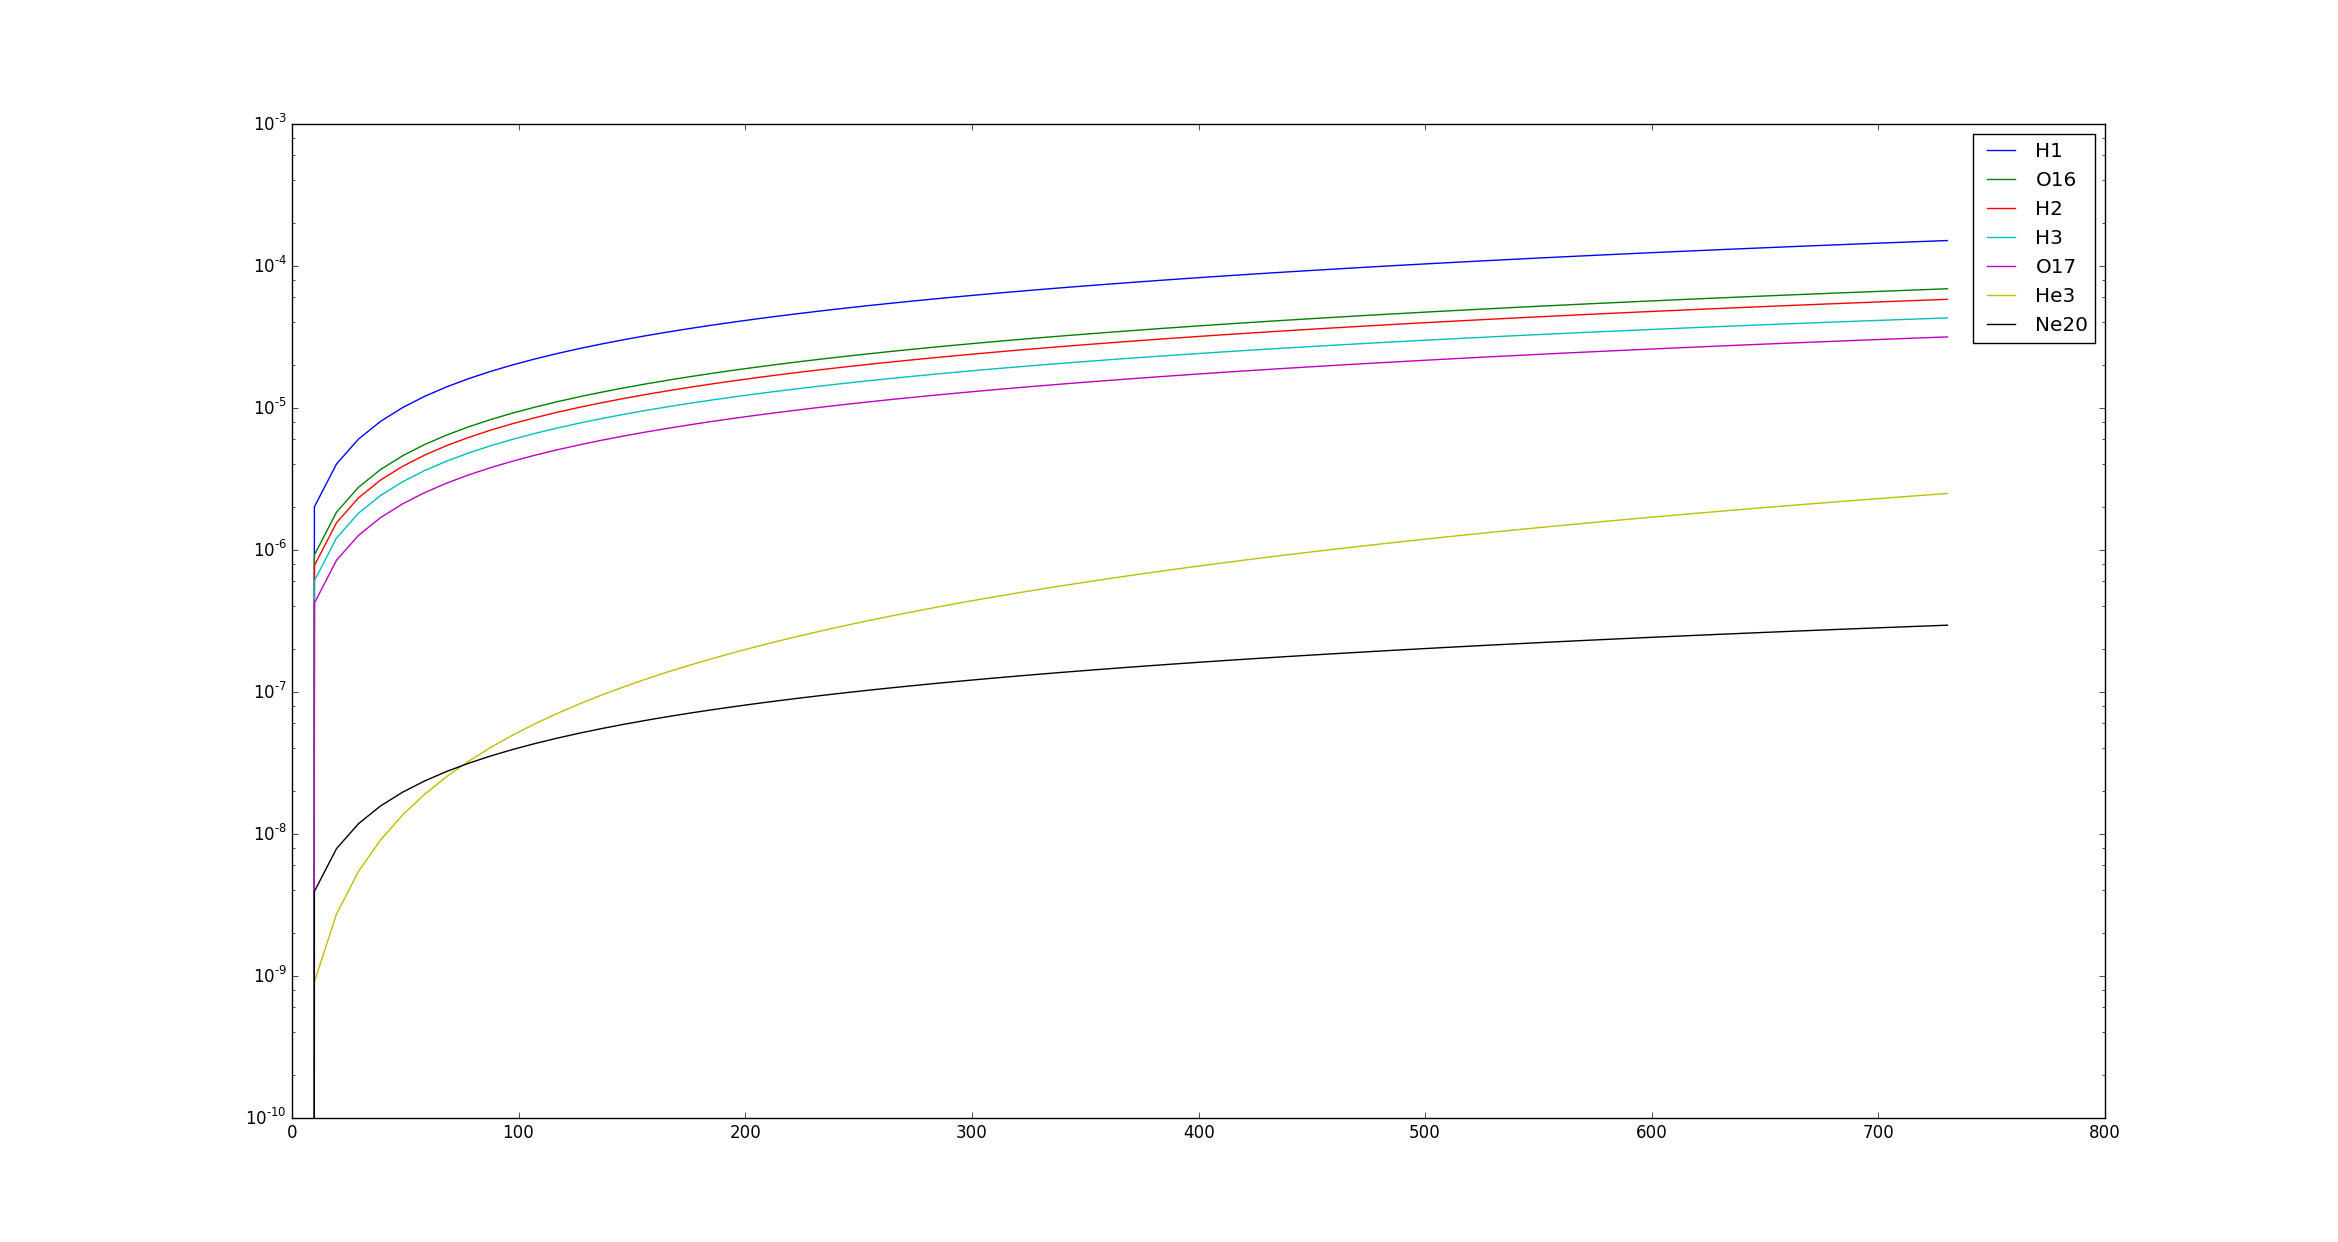
\includegraphics[width=.95\textwidth]{figures/2_2.png}
	\caption{Nuclides with next largest concentrations after irradiation from backward Euler method.}
\end{figure}

\clearpage

Next, the matrix exponential method is used to solve the depletion problem.

\script{../hw5}{Matrix Exponential Solution Method}{382}{394}{382}

\begin{figure}[h!]
	\centering
		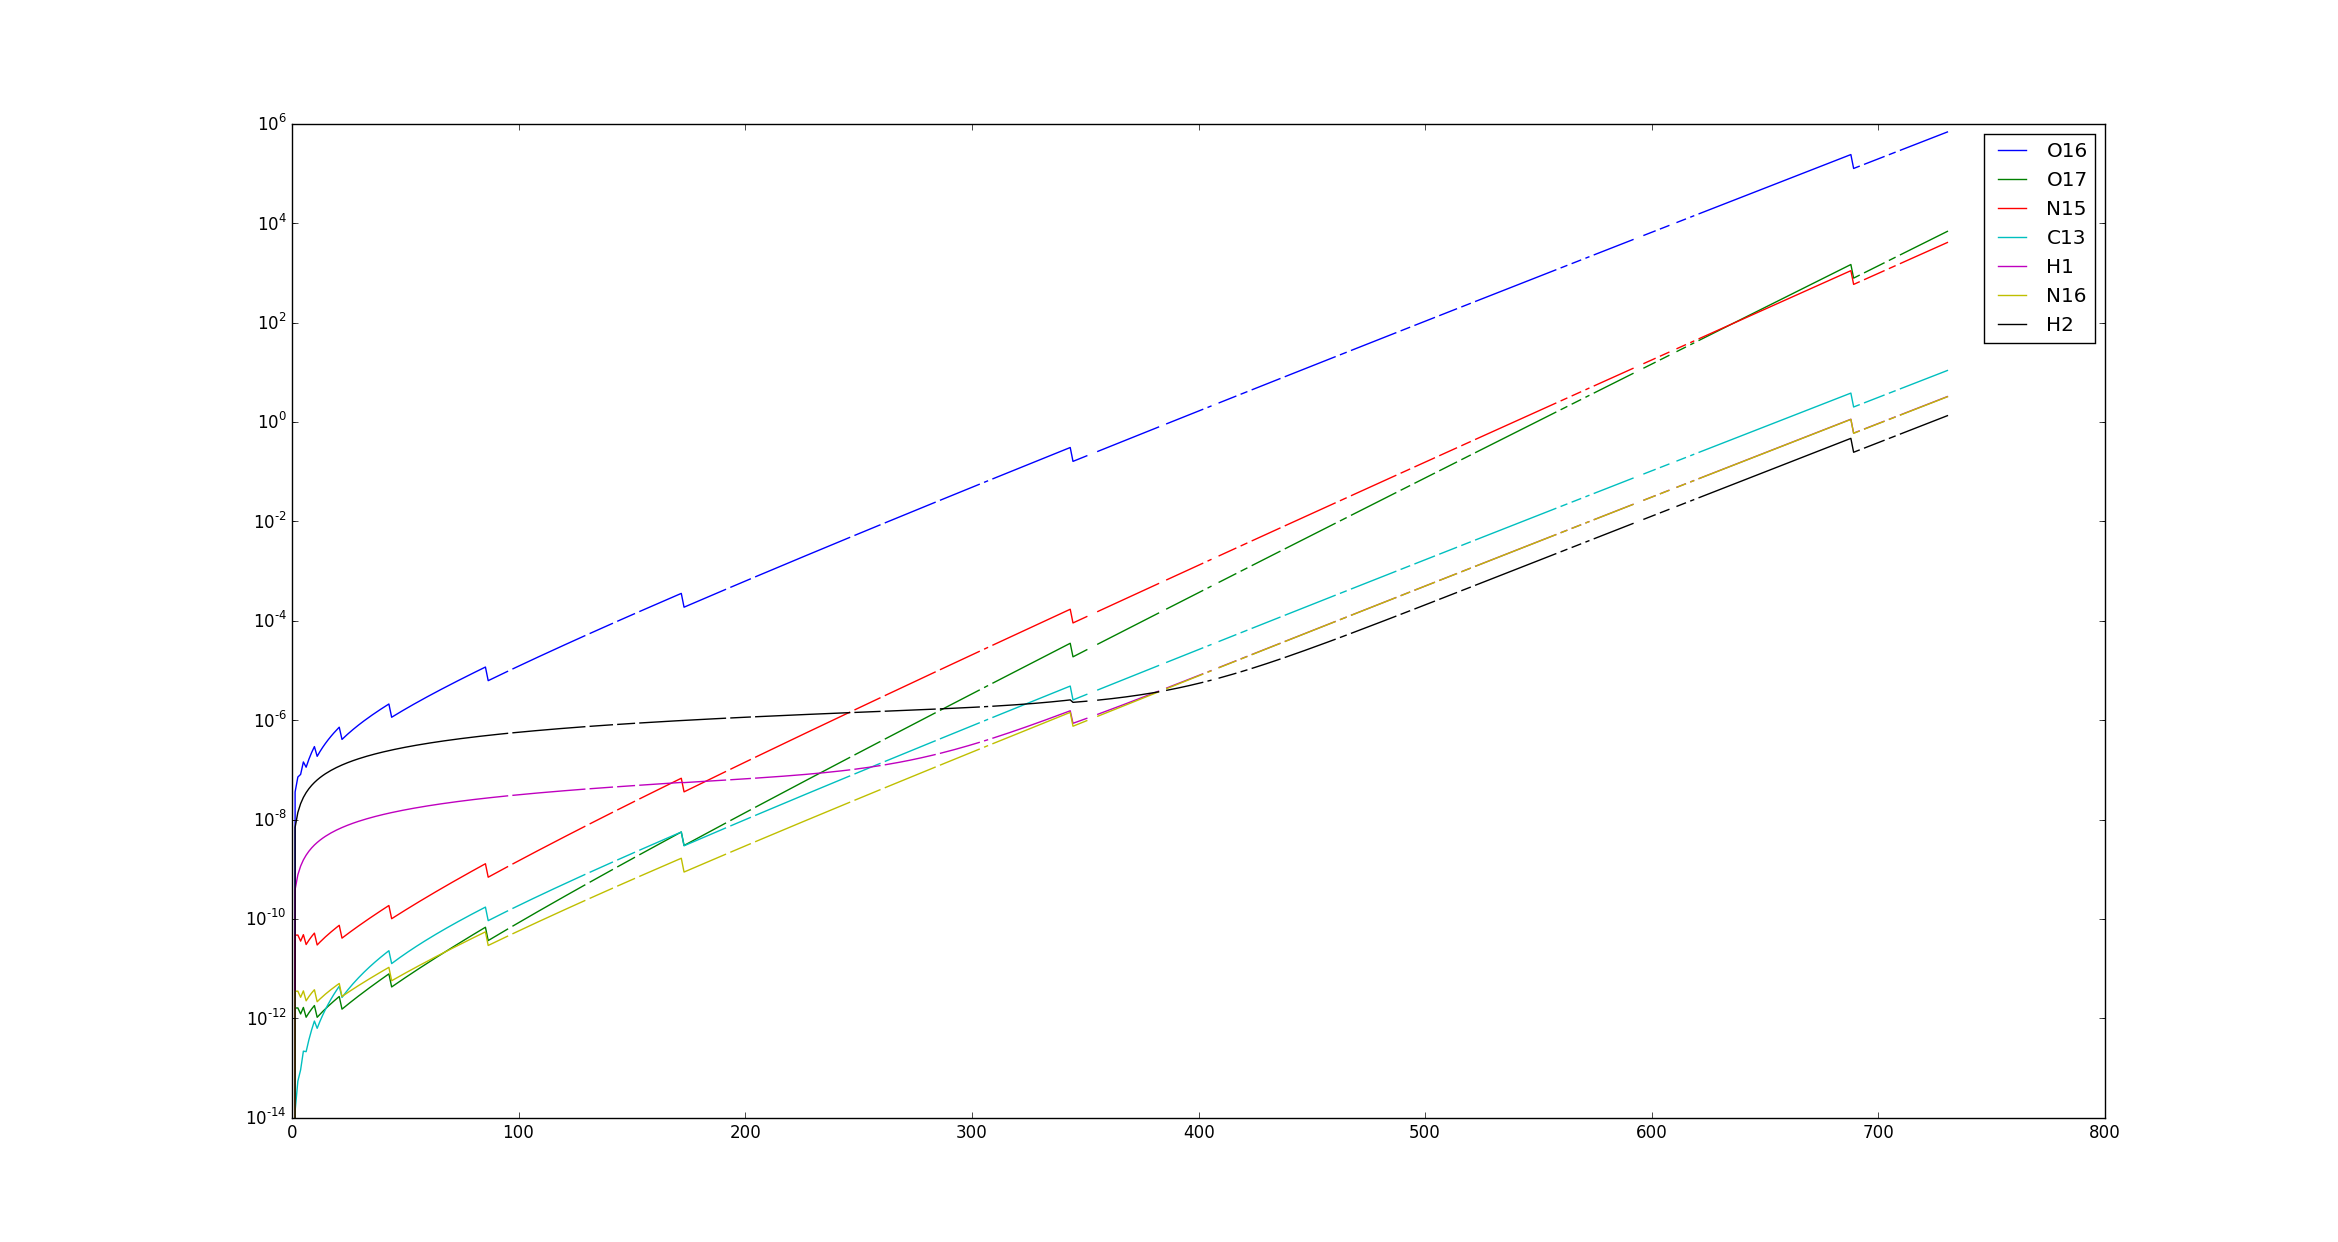
\includegraphics[width=.95\textwidth]{figures/2_3.png}
	\caption{Nuclides with largest concentration from matrix exponential method.}
\end{figure}

This method gives a tritium concentration of 0.0078297 kg tritium per kg FLiBe, a significant increase 
from the previous estimation.  The concentrations of all isotopes increases and goes above 1 suggesting that
there is a problem with how this method is solving the problem (more likely, just how I have set up the problem).
The kinks in the solution lend further evidence to the questionability of this method's implementation. Two 
solutions to fixing this implementation are to neglect some of the fast decaying (Be-8) isotopes and take shorter 
time steps.

\clearpage

The quadrature approximated matrix exponential method attempts to approximate the matrix exponential solution
by the best rational method producing quadrature points from residue calculus.

\script{../hw5}{Quadrature Approximated Matrix Exponential Solution Method}{413}{439}{413}

This method returns results for tritium concentration consistent with the backward Euler method
(4.312772 x 10$^5$ kg tritium per kg FLiBe) and maintains the dominance of the four natural
isotopes present, but results for built up isotopes are very erratic.  Though the concentration solutions
seem to oscillate around mean results similar to the backward Euler method, the error clearly dominates
this implementation.  Suggestions for making this method work are the same listed for matrix exponential 
method.

\begin{figure}[h!]
	\centering
		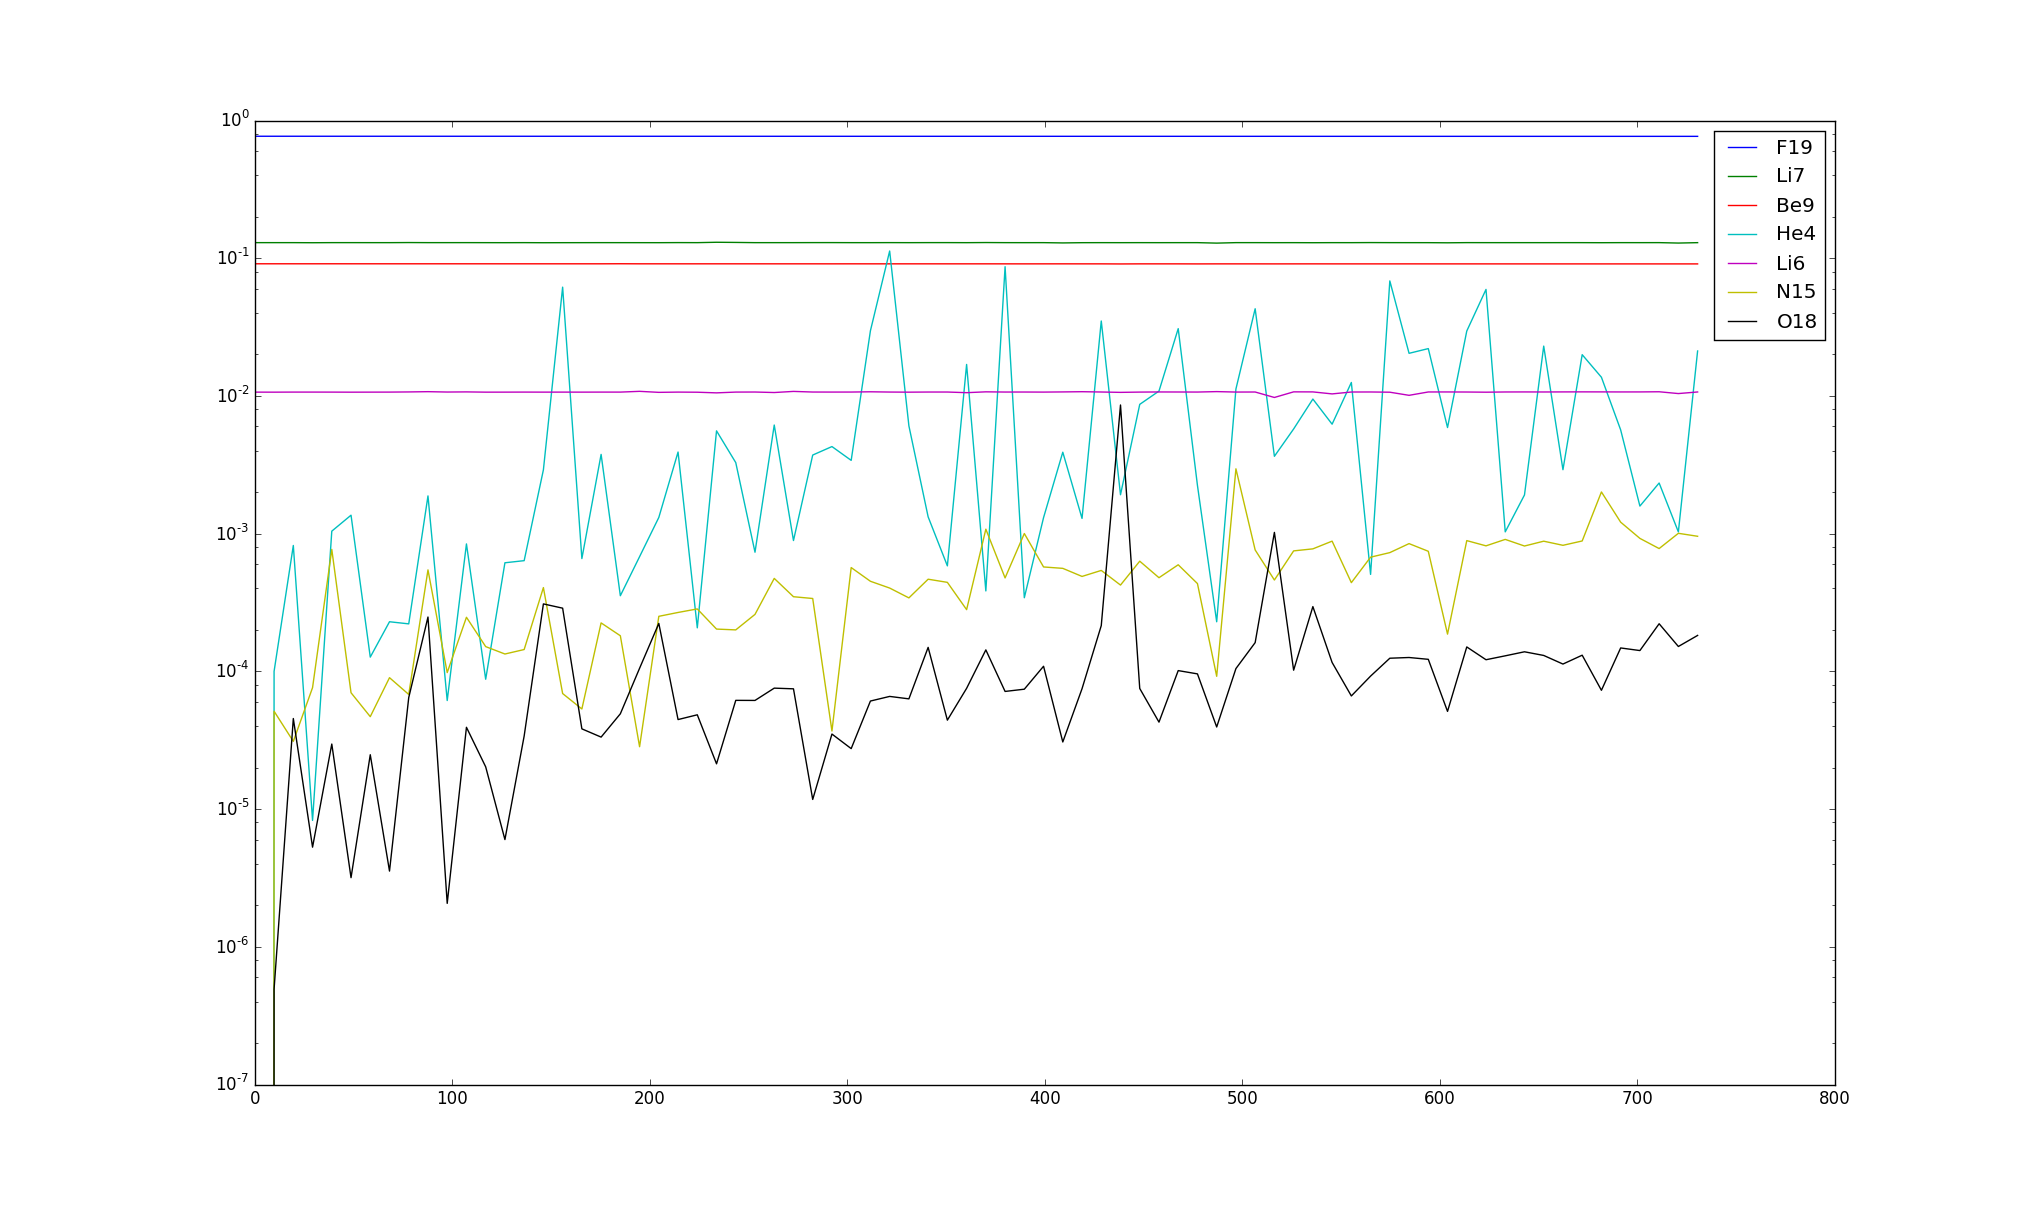
\includegraphics[width=.95\textwidth]{figures/2_4.png}
	\caption{Nuclides with largest concentration from quadrature matrix exponential method.}
\end{figure}

\begin{figure}[h!]
	\centering
		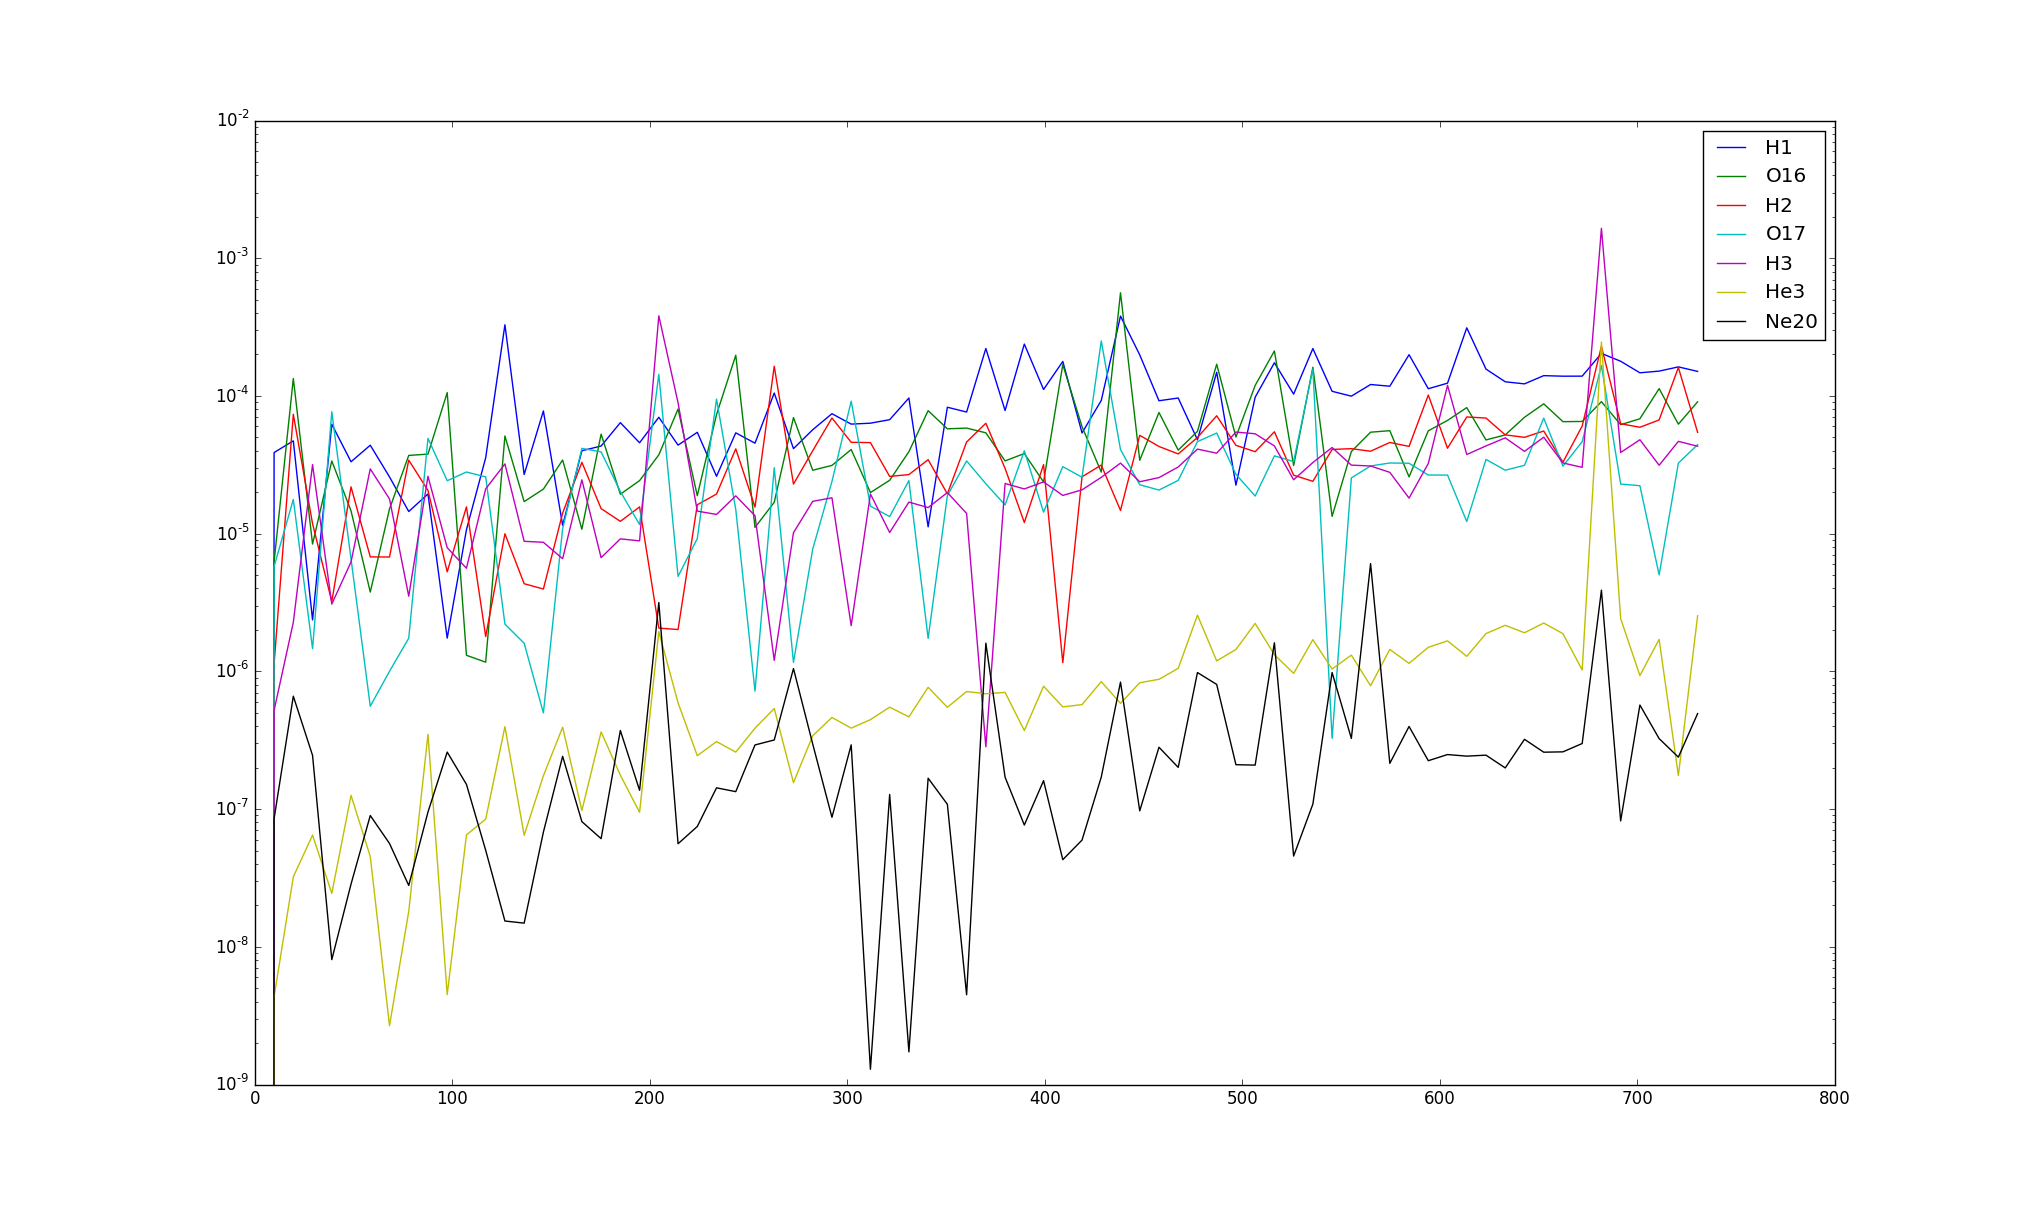
\includegraphics[width=.95\textwidth]{figures/2_5.png}
	\caption{Nuclides with next largest concentrations from quadrature matrix exponential method.}
\end{figure}

\clearpage

\end{homeworkProblem}

%----------------------------------------------------------------------------------------
%	PROBLEM 3
%----------------------------------------------------------------------------------------

% To have just one problem per page, simply put a \clearpage after each problem

\begin{homeworkProblem}

\script{../hw5}{Decay of Activation Products}{502}{549}{502}

\clearpage

Using the results from the backward Euler solution as initial quantities of materials and constructing a new 
matrix based solely on the decays of tracked nuclides, the backward Euler method is applied to
find how long it will take for the discharged FLiBe blanket to decay to below the activity of Brazil nuts
(444 Bq/kg).  The listing above demonstrates constructing the new decay matrix and solution method.
It ends up taking about 22,620 years for the isotopes present in the blanket to reach an activity of 420.15028 Bq/kg 
demonstrating the importance of considering long lived decay products even in fuels considered for "clean"
reactors utilizing fusion.

\begin{figure}[h!]
	\centering
		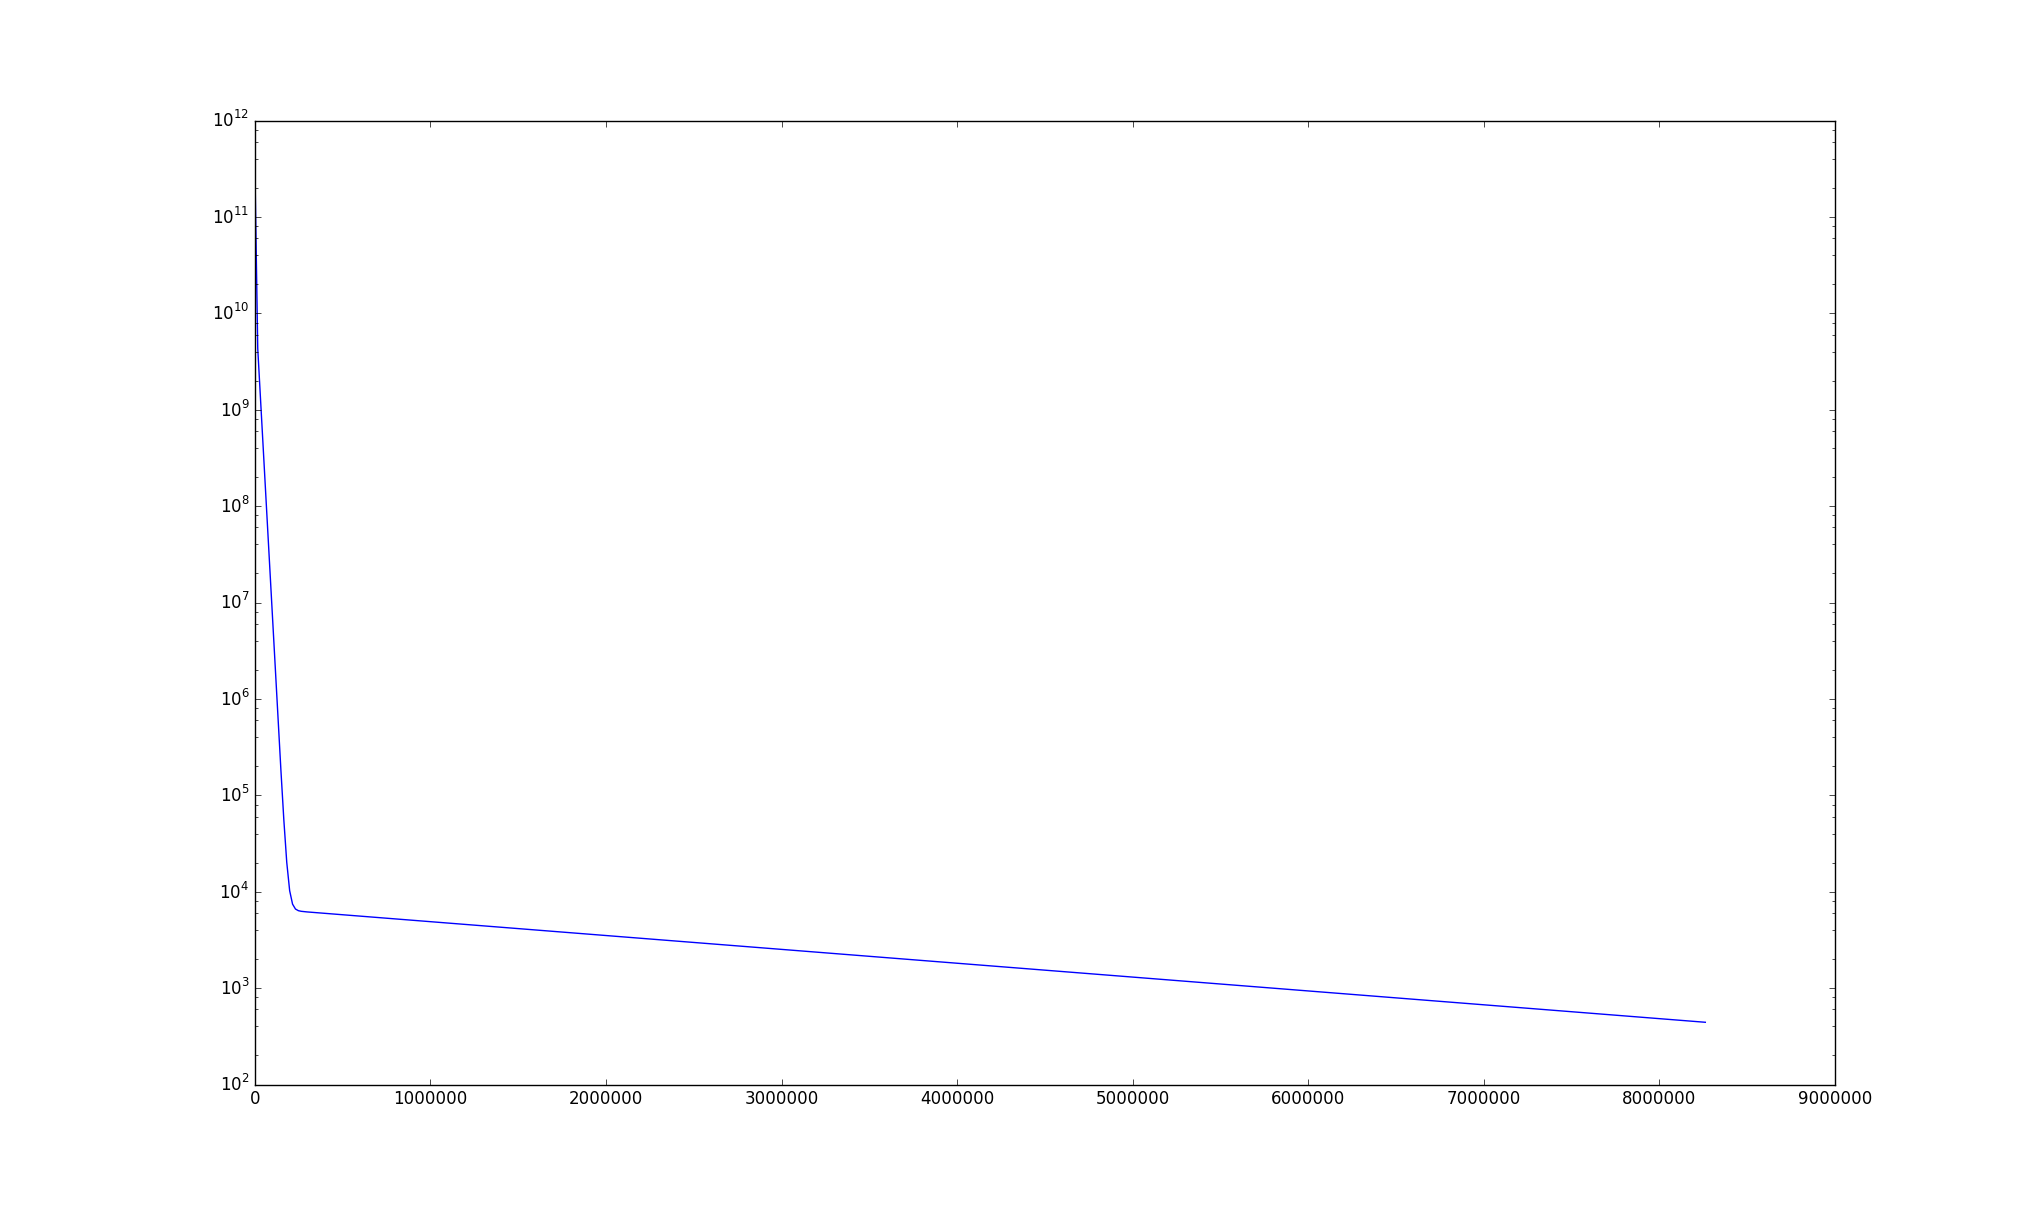
\includegraphics[width=.95\textwidth]{figures/3_1.png}
	\caption{Activity of FLiBe blanket plotted against days of decay.}
\end{figure}

\end{homeworkProblem}

\end{document}